    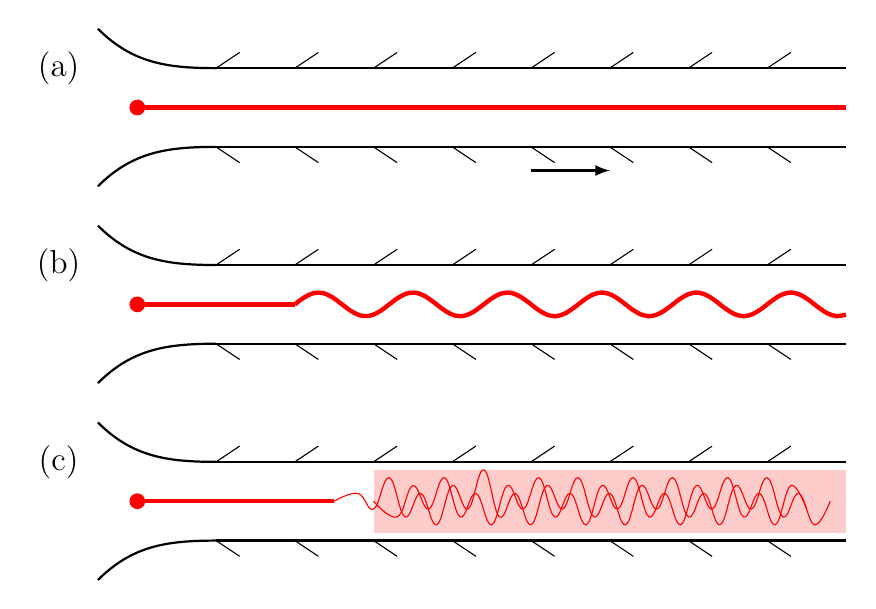
\begin{tikzpicture}[scale=1.0, >=latex]
        % --- SETTINGS ---
        \def\pipeL{8}
        \def\pipeH{1}
        \def\inletW{1.5}
        
        % =========================================
        % PART (a) LAMINAR FLOW (Top)
        % =========================================
        \begin{scope}[shift={(0, 4)}]
            % Pipe Walls
            \draw[thick] (0, \pipeH/2) -- (\pipeL, \pipeH/2);
            \draw[thick] (0, -\pipeH/2) -- (\pipeL, -\pipeH/2);
            
            % Inlet
            \draw[thick] (-\inletW, \pipeH/2 + 0.5) to[out=-45, in=180] (0, \pipeH/2);
            \draw[thick] (-\inletW, -\pipeH/2 - 0.5) to[out=45, in=180] (0, -\pipeH/2);
            
            % Wall Hatching
            \foreach \x in {0, 1, ..., 7} {
                \draw (\x, \pipeH/2) -- (\x+0.3, \pipeH/2 + 0.2);
                \draw (\x, -\pipeH/2) -- (\x+0.3, -\pipeH/2 - 0.2);
            }

            % Dye Streak (Straight)
            \draw[ultra thick, red] (-\inletW + 0.5, 0) -- (\pipeL, 0);
            \fill[red] (-\inletW + 0.5, 0) circle (0.1); 

            \node at (-2, 0.5) {\large (a)};
            % Flow Arrow
            \draw[->, thick] (4, -0.8) -- (5, -0.8);
        \end{scope}

        % =========================================
        % PART (b) TRANSITIONAL FLOW (Middle)
        % =========================================
        \begin{scope}[shift={(0, 1.5)}]
            % Pipe Walls
            \draw[thick] (0, \pipeH/2) -- (\pipeL, \pipeH/2);
            \draw[thick] (0, -\pipeH/2) -- (\pipeL, -\pipeH/2);
            
            % Inlet
            \draw[thick] (-\inletW, \pipeH/2 + 0.5) to[out=-45, in=180] (0, \pipeH/2);
            \draw[thick] (-\inletW, -\pipeH/2 - 0.5) to[out=45, in=180] (0, -\pipeH/2);
            
            % Wall Hatching
            \foreach \x in {0, 1, ..., 7} {
                \draw (\x, \pipeH/2) -- (\x+0.3, \pipeH/2 + 0.2);
                \draw (\x, -\pipeH/2) -- (\x+0.3, -\pipeH/2 - 0.2);
            }

            % Dye Streak (Sinusoidal Wave)
            \draw[ultra thick, red] (-\inletW + 0.5, 0) -- (1, 0); 
            \draw[ultra thick, red, smooth, domain=1:\pipeL, samples=60] plot (\x, {0.15*sin(300*(\x-1))});
            \fill[red] (-\inletW + 0.5, 0) circle (0.1);

            \node at (-2, 0.5) {\large (b)};
        \end{scope}

        % =========================================
        % PART (c) TURBULENT FLOW (Bottom) - IMPROVED
        % =========================================
        \begin{scope}[shift={(0, -1)}]
            % Pipe Walls
            \draw[thick] (0, \pipeH/2) -- (\pipeL, \pipeH/2);
            \draw[thick] (0, -\pipeH/2) -- (\pipeL, -\pipeH/2);
            
            % Inlet
            \draw[thick] (-\inletW, \pipeH/2 + 0.5) to[out=-45, in=180] (0, \pipeH/2);
            \draw[thick] (-\inletW, -\pipeH/2 - 0.5) to[out=45, in=180] (0, -\pipeH/2);
            
            % Wall Hatching
            \foreach \x in {0, 1, ..., 7} {
                \draw (\x, \pipeH/2) -- (\x+0.3, \pipeH/2 + 0.2);
                \draw (\x, -\pipeH/2) -- (\x+0.3, -\pipeH/2 - 0.2);
            }

            % Dye Streak Start (Straight -> Quick Transition)
            \draw[ultra thick, red] (-\inletW + 0.5, 0) -- (1.5, 0); 
            
            % Turbulent Region (Chaotic Mixing)
            % 1. Background Fill (Diffused Dye)
            \fill[red, opacity=0.2] (2.0, -0.4) rectangle (\pipeL, 0.4); 
            
            % 2. Chaotic Scribbles (Smooth curves instead of sharp lines)
            % We use 'plot coordinates' with tension to create fluid loops
            \draw[red, thin, smooth, tension=0.7] plot coordinates {
                (1.5, 0) (1.8, 0.1) (2.0, -0.1) 
                (2.2, 0.3) (2.4, -0.2) (2.6, 0.1) (2.8, -0.3)
                (3.0, 0.2) (3.2, -0.1) (3.4, 0.4) (3.6, -0.2)
                (3.8, 0.1) (4.0, -0.3) (4.2, 0.2) (4.4, -0.1)
                (4.6, 0.3) (4.8, -0.2) (5.0, 0.1) (5.2, -0.3)
                (5.4, 0.2) (5.6, -0.1) (5.8, 0.3) (6.0, -0.2)
                (6.2, 0.1) (6.4, -0.3) (6.6, 0.2) (6.8, -0.1)
                (7.0, 0.3) (7.2, -0.2) (7.4, 0.1) (7.6, -0.3)
                (7.8, 0)
            };
            
            % Add a second intertwining line to make it look "mixed"
            \draw[red, thin, smooth, tension=0.7] plot coordinates {
                (2.0, 0) (2.3, -0.2) (2.5, 0.2) (2.7, -0.1)
                (2.9, 0.3) (3.1, -0.2) (3.3, 0.1) (3.5, -0.3)
                (3.7, 0.2) (3.9, -0.1) (4.1, 0.3) (4.3, -0.2)
                (4.5, 0.1) (4.7, -0.3) (4.9, 0.2) (5.1, -0.1)
                (5.3, 0.3) (5.5, -0.2) (5.7, 0.1) (5.9, -0.3)
                (6.1, 0.2) (6.3, -0.1) (6.5, 0.3) (6.7, -0.2)
                (6.9, 0.1) (7.1, -0.3) (7.3, 0.2) (7.5, -0.1)
            };
            
            \fill[red] (-\inletW + 0.5, 0) circle (0.1);

            \node at (-2, 0.5) {\large (c)};
        \end{scope}

    \end{tikzpicture}
